\documentclass{report}
\usepackage{pgfplots}
\usepackage[europeanresistors]{circuitikz}
\usepackage{geometry}
\geometry{
 a4paper,
 total={170mm,257mm},
 left=20mm,
 top=20mm,
 }
\usepackage{amsmath}
\graphicspath{ {./images/} }
\title{P01 Report}
\author{Deepak Raj Gopal }
\date{February 2019}

\begin{document}

\maketitle
\chapter{Theoretical part}
\begin{center}

\begin{figure}
\centering
\begin{circuitikz}\draw
(0,0) to[battery] (0,4)
  to[resistor] (4,4) -- (4,0)
  to[resistor] (0,0)
;
\end{circuitikz}
\caption{Electrical Circuit Diagram}-0.275

\end{figure}

\end{center}


\section{Circuit Calculation}
Theoretical calculation of the
circuit \cite{lecture}
V1=1.1V-0.275

R1=2ohm
R2=2ohm\\
$VR = (R \times VT) / RT\\
$VR1=  (R1 \times V1) /$ RT = 1.1V\\
$VR2= (R2 \times V2)/ RT = -0.275 V\\




 



\begin{table}[h!]
\begin{center}
\begin{itemize}
\color{green}
\caption\item {Table for resistance and voltage}
\end{itemize}
\begin{tabular}{ |c|c| } 
 \hline
 V1 & 1.1  \\ 
 \hline\hline
 R1 & 2ohm  \\ 
 \hline\hline
 R2 & 2ohm \\
 \hline\hline
 UR1 & 1.1V  \\ 
 \hline\hline
 UR2 & -0.275V \\
 \hline
\end{tabular}
\end{center}

 \end{table}
 
 \begin{center}
\end{center}

\chapter{Practical part}
Practical Calculation
\section{‘Working on with GEDA programs'}
\subsection{'Working with gschem'}
\begin{figure}[hbt!]
 \centering
 \caption{Circuit Diagram created in gscehm}
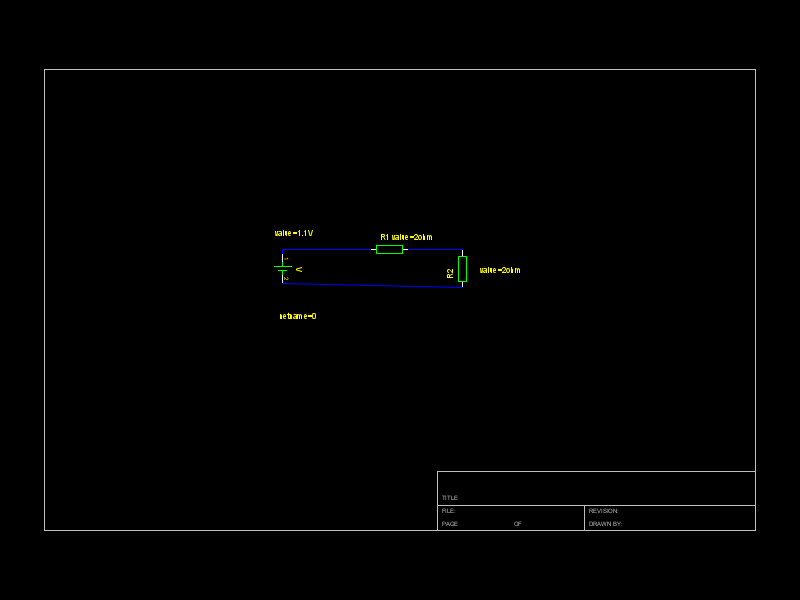
\includegraphics[width=\textwidth]{01.png}
 \end{figure}
\subsection{'Work with gnetlist'}

\begin{figure}[hbt!]
 \centering
  \caption{The plotted graph after using ngspice}
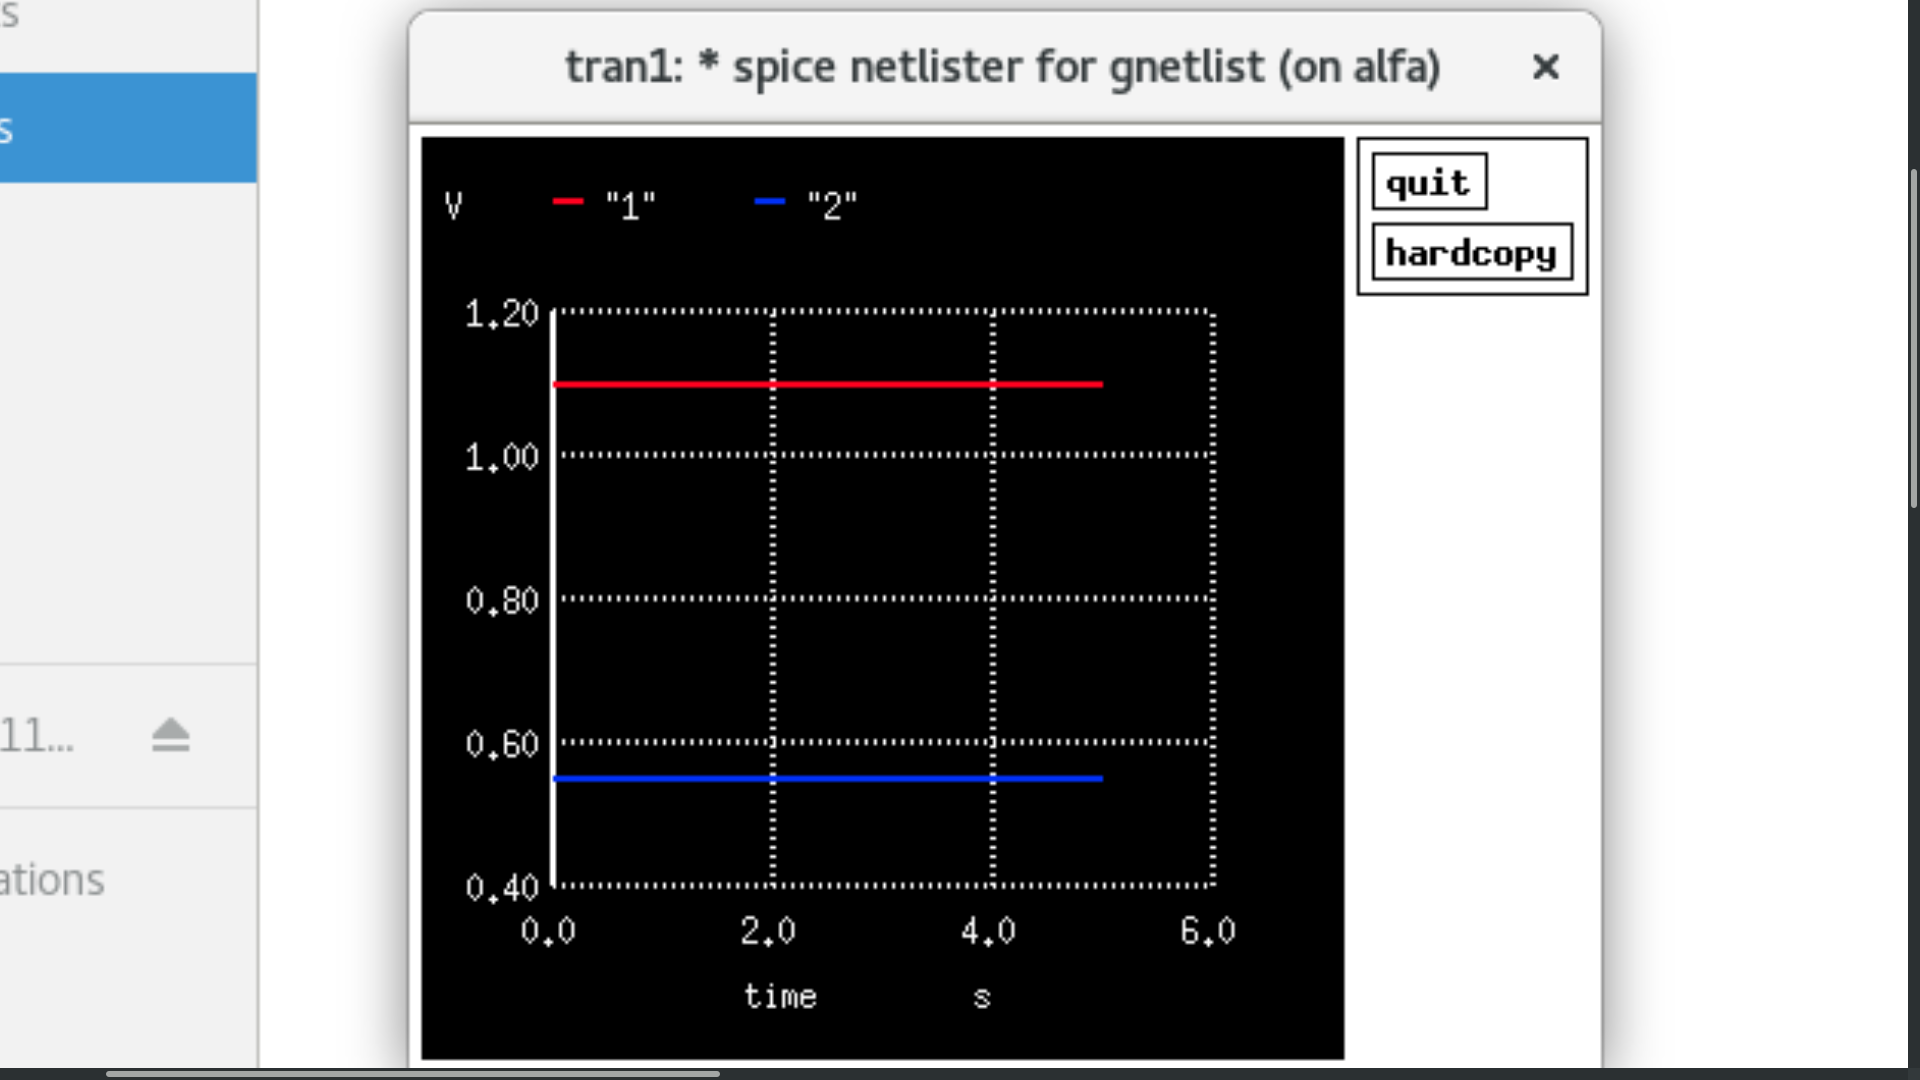
\includegraphics[width=\textwidth]{03.png}
 \end{figure}
 

\begin{center}
\begin{tikzpicture}
\begin{axis}[axis lines = left,
    xlabel = $R2$,
    ylabel = $U(R2)$,
    xmin=0,
    xmax=14]
    \addplot [green, very thick]{1.1*x(x+3)};
\end{axis}
\end{tikzpicture}
\end{center}
\begin{thebibliography}{2}

\bibitem{lecture}
lecture notes and screenshots
\end{thebibliography}

\end{document}
